\documentclass[12pt]{article}
\usepackage{amssymb,amsmath}
\usepackage{anyfontsize}
\thispagestyle{empty}
\usepackage{tikz}
\usetikzlibrary{calc}
\usepackage{setspace}
\usepackage{graphicx}
\usepackage[margin=0.65in]{geometry}
\usepackage{float}
\usepackage[letterspace=150]{microtype}


\begin{document}

%Border

\begin{tikzpicture}[overlay,remember picture]
\draw [line width=3pt,rounded corners=0pt,]
    ($ (current page.north west) + (1.25cm,-1.25cm) $)
    rectangle
    ($ (current page.south east) + (-1.25cm,1.25cm) $);       
\end{tikzpicture}
\begin{center}
\includegraphics[scale=.40]{RUMAlogo.png}
  
  presents... 

  \vspace{2mm} 
\begin{spacing}{1}
{\fontsize{40}{44}\selectfont  \textsc{
$e^x$}} \end{spacing}
 

~~\\
\begin{spacing}{1.5}
{\fontsize{24}{24} \selectfont A Lecture by Professor Matthew
  Russell}  \end{spacing}  
\large Dept. of Mathematics, Rutgers University \\~~\\

\normalsize
\textsc{Abstract:}

\Large
We will explore the history of the exponential function $e^x$.
\\

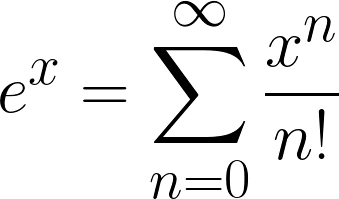
\includegraphics[scale=.45]{CodeCogsEqn.png}

\vspace{2mm} 
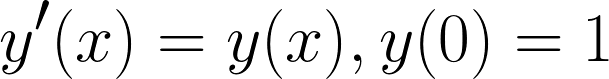
\includegraphics[scale=.45]{CodeCogsEqn(1).png}

\vspace{2mm} 
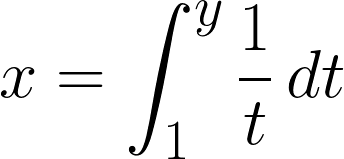
\includegraphics[scale=.45]{CodeCogsEqn(2).png}

\vspace{2mm} 
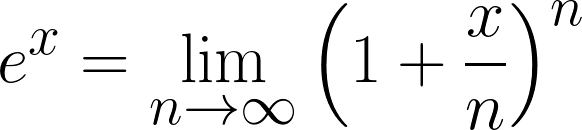
\includegraphics[scale=.45]{CodeCogsEqn(3).png}

\vspace{5mm} 
\Huge   \textsc{Tuesday\\February 11, 2020 \\Hill 423 at 7:00
  pm}

\vspace{2mm}
\large
\emph{*Pizza and refreshments will be served}
\end{center}

\begin{center}
  \large  Join our email list! Email us at math.ruma@gmail.com, or
go to bit.ly/RUMA2019.\\
\end{center}



\end{document}